\documentclass{article}
\usepackage[a4paper, total={6in, 8in}]{geometry}
\usepackage{graphicx} % Required for inserting images
\usepackage{amssymb}
\usepackage{amsmath}
\usepackage{amsfonts}
\usepackage{extarrows}
\usepackage{soul}
\usepackage{enumitem}
\usepackage{varwidth}
\usepackage[T1]{fontenc}

\author{}
\date{}
\title{Correction TD1 Physique quantique}

\begin{document}
\maketitle

\noindent\textbf{Exercice de cours : Catastrophe ultraviolette}\newline
\indent Le corps noir est l'objet théorique suivant : il absorbe parfaitement la totalité de l'énergie électromagnétique qu'il reçoit et, atteignant l'équilibre thermique à une température T, la restitue entièrement sous forme d'un rayonnement thermique constitué d'un spectre de longueurs d'onde $\lambda$, rayonnées chacune à une intensité, donnée par la fonction u($\lambda$, T), appelée densité spectrale d'énergie.\newline
\indent La thermodynamique classique a proposé de décrire le rayonnement du corps noir en considérant les molécules comme de petits oscillateurs, rayonnant chacun une énergie E avec une certaine probabilité. La physique classique propose que l'énergie rayonnée E prend ses valeurs dans $[0;+\infty]$ ; des valeurs donc continues. On note <E> l'énergie moyenne d'un oscillateur.\newline\newline
\noindent\textbf{Partie 1 : Descritpion par la loi de Rayleigh-Jeans (Énergie continue)}\newline
Dans le cadre de la thermodynamique classique, la loi de Rayleigh-Jeans aboutit à l'expression suivante pour la densité spectrale d'énergie:
\[
    u(\lambda,T) = \frac{8\pi}{c\lambda^{2}} \langle E \rangle
\quad
\begin{varwidth}{\displaywidth}
    \begin{itemize}[nosep]
        \item u: densité spectrale (W$\cdot$m$^{3}$)
        \item c: célérité de la lumière dans le vide (3$\times$10$^{8}$m$\cdot$s${-1}$)
    \end{itemize}
\end{varwidth}
\]

\noindent
L'énergie moyenne <E> d'un oscillateur se calcule de la manière suivante:
\[
    \langle E \rangle = \frac{\int_{0}^{+\infty} Ee^{-\frac{E}{k_{B}T}}dE}{\int_{0}^{+\infty} e^{-\frac{E}{k_{B}T}}dE}
\quad
\begin{varwidth}{\displaywidth}
    \begin{itemize}[nosep]
        \item $k_{B}$: constante thermodynamique
        \item T : température du rayonnement
    \end{itemize}
\end{varwidth}
\]

\noindent
Le numérateur représente l'intégrale de la densité de probabilité de l'énergie E, et le dénominateur permet de normaliser le résultat.\newpage
\begin{enumerate}
    \item Montrer que le terme $\langle E \rangle$ a pour valeur $k_{B}T$, en utilisant une intégration par parties. \newline
    Posons Nm et D tel que $\langle E \rangle = \frac{Nm}{D}$\newline
    \[ D = \int_{0}^{\infty} e^{-\frac{E}{k_{B}T}} dE = [-k_{B}T\times e^{-\frac{E}{k_{B}T}}]_{0}^{\infty} = -k_{B}T(0-1) = k_{B}T \]
    \begin{flalign*}
        Nm & = \int_{0}^{\infty} E\times e^{-\frac{E}{k_{B}T}}dE, \text{ par intégration par parties, on obtient} &\\
           & = \left[-k_{B}T\times E\times e^{-\frac{E}{k_{B}T}}\right]_{0}^{\infty} - \left(\int_{0}^{\infty} -k_{B}T\times e^{-\frac{E}{k_{B}T}}dE\right) &\\
           & = k_{B}T \left[-Ee^{-\frac{E}{k_{B}T}}\right]_{0}^{\infty} + k_{B}T\left[-k_{B}Te^{-\frac{E}{k_{B}T}}\right]_{0}^{\infty} &\\
           & = k_{B}T[0-0] - (k_{B}T)^{2} \left[e^{-\frac{E}{k_{B}T}}\right]_{0}^{\infty} &\\
           & = -(k_{B}T)^{2} [e^{-\infty} - e^{0}] &\\
           & = -(k_{B}T)^{2} (0-1) &\\
        Nm & = (k_{B}T)^{2}
    \end{flalign*}
    Donc $\langle E \rangle = \frac{Nm}{D}$ = $\frac{(k_{B}T)^{2}}{k_{B}T}$ = $k_{B}$T\newline\newline

    L'énergie totale du rayonnement émis par le corps noir est donnée par l'intégration de la densité d'énergie sur toutes les longueurs d'ondes:
    \[ U(\lambda,T) = \int_{0}^{+\infty} u(\lambda,T)d\lambda\]

    U($\lambda$,T) est l'intensité rayonnée par le corps noir (en W$\cdot$m$^{2}$)
    \item Expliquer à partir de cette intégrale pourquoi la loi de Rayleigh-Jeans a marqué un tournant nommé "Catastrophe ultraviolette".\newline
    \begin{flalign*}
        \int_{0}^{+\infty} u(\lambda,T)d\lambda & = \int_{0}^{\infty} \frac{8\pi}{c\lambda^{2}}\times k_{B}T d\lambda &\\
                                        & = \frac{8\pi}{c}\times k_{B}T \times \int_{0}^{\infty} \frac{1}{\lambda^{2}}d\lambda &\\
                                        & = \frac{8\pi}{c}\times k_{B}T \times \left[\frac{-1}{\lambda}\right]_{0}^{\infty}
    \end{flalign*}\newline
    $\Longrightarrow$ $\lambda \rightarrow 0 \Longrightarrow$ U($\lambda$,T) diverge.
\end{enumerate}

\newpage
\noindent\textbf{Partie 2: Descritpion par la loi de Planck (Énergie discontinue)}\newline
Nous allons maintenant nous intéresser à la loi de Planck, qui a proposé de corriger la loi de Rayleigh-Jeans en introduisant la quantification de l'énergie du système corps noir : le terme <E> est alors calculé en supposant que l'énergie E d'un oscillateur ne peut prendre qu'un nombre discret de valeurs, multiples d'une énergie $E_{0}$.
\begin{enumerate}
    \setcounter{enumi}{2}
    \item Réécrire la relation donnant $\langle E \rangle$ dans ces conditions.\newline
    Proposition de Max-Planck: E = n$E_{0}$ (quantificateur de l'énergie) qui corrige la divergence de la densité spectrale u($\lambda$,T) pour les faibles longueurs d'ondes (UV).
    \[ \langle E \rangle = \frac{\Sigma_{n=1}^{+\infty} nE_{0} e^{-\frac{nE_{0}}{k_{B}T}}}{\Sigma_{n=1}^{+\infty} e^{-\frac{nE_{0}}{k_{B}T}}} \]
    \item Calculer ce terme, en utilisant un résultat sur les suites géométriques au dénominateur, puis en remarquant un lien de dérivation entre le dénominateur et le numérateur.\newline
    \underline{Calcul de $\langle$E$\rangle$:} \[ \langle E \rangle = \frac{\Sigma_{n=1}^{+\infty} nE_{0} e^{-\frac{nE_{0}}{k_{B}T}}}{\Sigma_{n=1}^{+\infty} e^{-\frac{nE_{0}}{k_{B}T}}} = \frac{Nm}{D} \]
    \begin{flalign*}
        D & = \Sigma_{n=1}^{+\infty} e^{-\frac{nE_{0}}{k_{B}T}} = \Sigma_{n=1}^{+\infty} \left(e^{-\frac{nE_{0}}{k_{B}T}}\right)^{n} &\\
          & = \Sigma_{n=1}^{+\infty} q^{n} \text{ (avec } q = e^{-\frac{E_{0}}{k_{B}T}} \text{)} = \lim_{n\to +\infty} q^{n} &\\
          & = \lim_{n\to +\infty} \frac{1-q^{n}}{1-q} &\\
        D & = \frac{1}{1-q} = \frac{1}{1-e^{-\frac{E_{0}}{k_{B}T}}}
    \end{flalign*}\newline

    \begin{flalign*}
        Nm & = \Sigma_{n=1}^{+\infty} nE_{0} e^{-\frac{nE_{0}}{k_{B}T}} &\\
           & = 
    \end{flalign*}

    \item On obtient donc la densité spectrale d'énergie suivante :
    \[ u(\lambda,T) = \frac{8\pi}{c\lambda^{2}}<E> = \frac{8\pi}{c\lambda^{2}} \times \frac{E_{0}}{e^{\frac{E_{0}}{k_{B}T}}-1} \text{ avec $E_{0}$ un quanta (plus petite quantité indivisible d'énergie)} \] 
    Pour corriger la loi de R-J, il faut corriger la divergence u($\lambda$,T) pour les petites longueurs d'ondes.\newline
    Justifier la proposition de Planck: $E_{0} = \frac{hc}{\lambda}$ avec h la constante de Planck.\newline
    \begin{figure}[h]
        \centering
        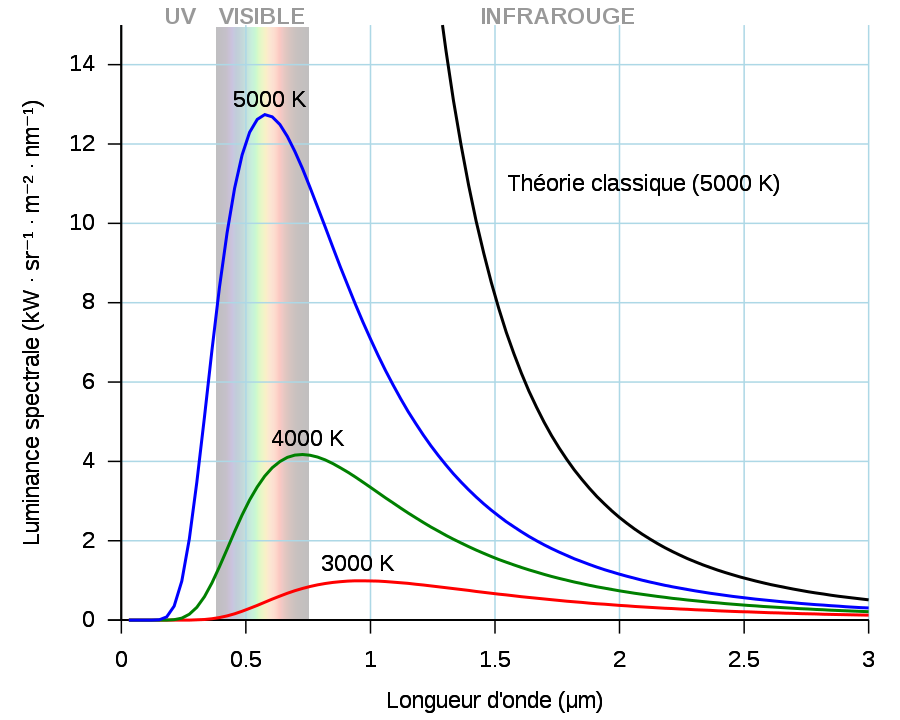
\includegraphics[scale=0.3]{catastrophe_ultraviolette.png}
        \caption{Spectre du rayonnement du corps noir (intensité du rayonnement en fonction de la longueur d'onde) pour des températures données (couleurs : modèle de Planck ; noir : modèle de Rayleigh-Jeans)}
    \end{figure}

    \indent\textit{Remarques:}\textit{Avec la loi de Planck, l'on trouve une énergie totale rayonnée U(T)$\alpha$T$^{4}$ , ce qui est en accord avec les observations, et revient à la loi de Stefan-Boltzman, antérieure à la catastrophe ultraviolette.}
\end{enumerate}
\end{document}
